This chapter discusses the details of display protocols. Firstly, it provides a general discussion of how common display protocols work to send pixel data to a display system (e.g. a television). Then, it discusses how these protocols are utilized within IRSP technology.

\section{Classical Display Protocols}
    \label{sec:classical_display_protocols}

    Display specifications such as DSI\cite{HDMIForum2017}, DVI\cite{DDWG1999}, HDMI\cite{HDMIForum2018}, and DisplayPort\cite{VESA2016} are the backbone of consumer electronic display devices. They are utilized in a plethora of devices ranging from televisions, monitors, laptops, smart phones, to embedded devices such as point of sale (POS) terminals. Increasingly, they are being utilized in the ever increasing smart display market for applications such as registration, product menus, smart watches, etc.

    These generally provide a standardized feature-set, or display protocol, that is rooted in classical analog video specifications (e.g. VGA, Composite)\cite{NIAnalog} that utilize scan lines\cite{Neal1998}. Scan lines are used to provide video timing information in order to synchronize a display to a given refresh rate. Each scan line consist of an active video region followed by a horizontal blanking period. After all active video scan lines are displayed, a vertical synchronization region is used to indicate the end of a frame.

    %FIXME add crosssectional blowout chart

    An overview of this is shown in Figure~\ref{fig:display_protocol_timing_overview}. The region shown in green is the pixel data for the active video region of the display. It is of size $h_a\cdot v_a$ which represents the number of pixels to display, for example, 1920 by 1080 for a HDTV high-definition video mode\cite{MythTVWebsite}. The blanking time regions denote pixel data that is sent but not displayed\footnote{Typically data lines are held low during this period, but sometimes they are used for out-of-band communication to send other information such as audio encoding.}. A scan line consist of pixels made up of the $h_a+h_{fp}+h_{sp}+h_{bp}$ regions. These are the horizontal active size, the horizontal front porch, the horizontal sync pulse; and the horizontal back porch respectively. $v_a$, the vertical active size, indicates the number of scanlines that make up the active region of the display. The vertical blanking period makes up multiple scanlines and consist of $v_{fp}+v_{sp}+v_{bp}$ scanlines. These are the vertical front porch before the vsync pulse, the vertical sync pulse, and the vertical back porch respectively. Sync pulses are generally active low, meaning that during active display a sync signal is high as shown in the diagram. Note, that this terminology is consistent with the VESA Coordinated Video Timings (CVT) Standard\cite{VESA2013}.

    Figure~\ref{fig:display_protocol_line_cross} shows a closeup view of signal lines during the active region of display for two scan lines\footnote{The active pixel count is proportionally smaller to blanking regions than in real modes for illustration purposes.}. A data enable signal denoted by $enable$ is high during the active region shown in green. Following this, it goes low for a period of time denoted by the $h_{fp}+h_{sp}+h_{bp}$ regions. The horizontal sync signal goes low only in the region shown in yellow between the front porch and back porches. This process repeats for all scan lines. Once the last active region pixel is drawn, the enable signal will stop going high during the vertical synchronization period.

    %FIXME: Fix discussion of DP not using fucking backwards compatibility shitty hdmi fucking mode
    %FIXME: Talk about CC in the vertical blanking

    Figure~\ref{fig:display_protocol_full_cross} shows a closeup view of signal lines during the transition into the vertical synchronization period\footnote{The blanking regions are less scanlines than in real modes for illustration purposes.}. The region donated by $v_a$ indicates the end of the video active region of the display which occurs toward the end of a frame. After the active video region, all data has been drawn to a display. The region denoted by $v_{fp}+v_{sp}+v_{bp}$ is the vertical blanking or vsync period during which no active video data is sent; therefore, data enable denoted by $enable$ is always low during this period. Before the vertical sync pulse period denoted by $v_{sp}$ occurs, a vertical front porch period denoted by $v_{fp}$ occurs. After the vertical sync pulse, a vertical back porch region $v_{bp}$ occurs. Following this, the beginning of the next frame begins after the $v_{bp}$ region.

    \begin{figure}[H]
        \centering
        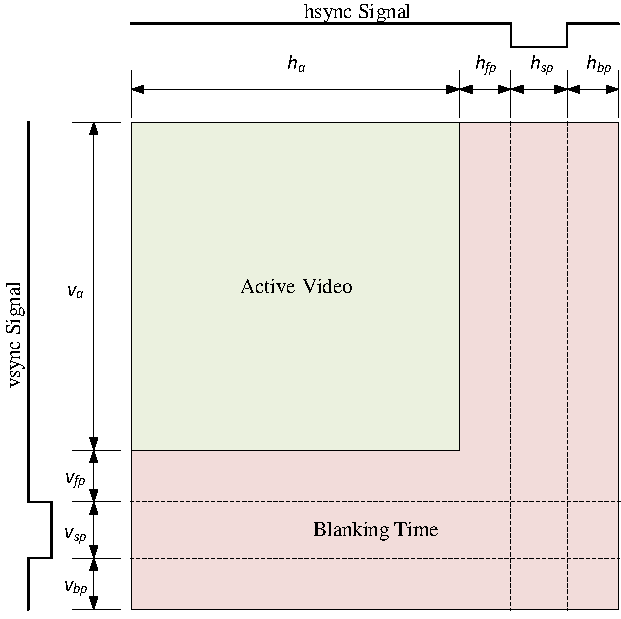
\includegraphics[width=1.0\textwidth]{fig/display_timing_overview.pdf}
        \caption{Display Protocol Timing Overview}
        \label{fig:display_protocol_timing_overview}
    \end{figure}

    \begin{figure}[H]
        \centering
        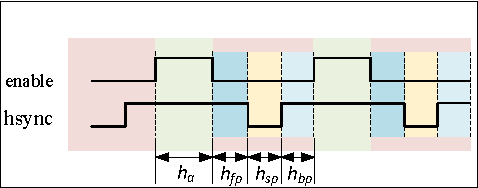
\includegraphics[width=1.0\textwidth]{fig/display_timing_line_cross.pdf}
        \caption{Display Protocol Horizontal Signal Cross Section Timing}
        \label{fig:display_protocol_line_cross}
    \end{figure}

    \begin{figure}[H]
        \centering
        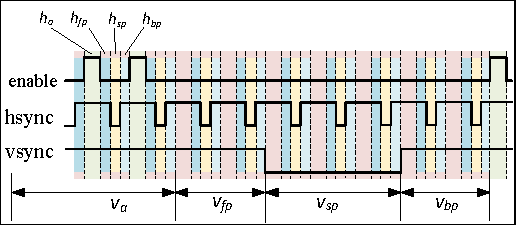
\includegraphics[width=1.0\textwidth]{fig/display_timing_full_cross.pdf}
        \caption{Display Protocol Full Signal Cross Section Timing}
        \label{fig:display_protocol_full_cross}
    \end{figure}

    Equations~\ref{eq:l_h}~through~\ref{eq:f_t} show the relationship between between the different regions of a display and the frequency or refresh rate. In Equation~\ref{eq:l_h}, $l_h$ denotes the scan line size of a display, or total horizontal width, which is made up of the horizontal active and horizontal porch region pixels of a display. In Equation~\ref{eq:l_v}, $l_v$ denotes the total vertical width of a display, which is made up the vertical active and vertical porch region pixels of a display. In Equation~\ref{eq:f_f}, each pixel is sent at a rate denoted by $f_p$, the pixel frequency (also called the pixel clock)where the result $f_f$ denotes the frame frequency or frame rate of a display. This is simply the pixel frequency over the total number of pixels (video active and porches) of a display. In Equation~\ref{eq:p_t}, $p_t$ denotes the time period a single pixel takes to send. In equation~\ref{eq:f_t}, $f_t$ denotes the time period for an entire frame.


    \begin{equation}
        l_h=h_a+h_{fp}+h_{sp}+h_{bp}
        \label{eq:l_h}
    \end{equation}
    \begin{equation}
        l_v=v_a+v_{fp}+v_{sp}+v_{bp}
        \label{eq:l_v}
    \end{equation}
    \begin{equation}
        f_f={\frac{f_p}{l_h \cdot l_v}}
        \label{eq:f_f}
    \end{equation}
    \begin{equation}
        p_t={\frac{1}{f_p}}
        \label{eq:p_t}
    \end{equation}
    \begin{equation}
        f_t={\frac{1}{f_f}}
        \label{eq:f_t}
    \end{equation}

    %FIXME: example modeline
    To illustrate, let us look at the display modeline generated using the VESA Coordinated Video Timing (CVT) standard shown in Table~\ref{tbl:modeline_example}. This modeline operates a total frame frequency of approximately \mbox{30 Hz}. The pixel clock 79.75, denoted in red, is specified in megahertz. The horizontal pixels, denoted in blue; are the horizontal display width, the horizontal sync start, the horizontal sync end, and the horizontal total pixels respectively. The vertical pixels (measured in lines), denoted in green; are the vertical display height, the vertical sync start, the end of vertical sync end, and the horizontal total pixels respectively. The sync pulse polarities, denoted in yellow; indicate whether a given sync pulse is active low or active high. A minus symbol indicates active low and a plus symbol indicates active high. The terminology for these modeline parameters comes from The X Window System\cite{TheOpenGroup2020}, a commonly utilized windowing system in the Linux family of operating systems where the parameters, while equivalent, are specified in a different format from the VESA standards. Equations~\ref{eq:h_a_solve}~and~\ref{eq:v_a_solve} show the relationship between the X Window System parameters and the VESA parameters.

    \begin{table}
        \small
        \setlength\tabcolsep{2pt}
        \begin{tabular}{| c c c c c |}
            \hline
                \textbf{\footnotesize Name} & \begin{tabular}{c} \textbf{\footnotesize Pixel} \\ \textbf{\footnotesize Clock} \\ \textbf{\footnotesize (MHz)} \end{tabular}
                & \begin{tabular}{c} \textbf{\footnotesize Horizontal} \\ \textbf{\footnotesize Parameters} \\ \textbf{\footnotesize (pixels)} \end{tabular}
                & \begin{tabular}{c} \textbf{\footnotesize Vertical} \\ \textbf{\footnotesize Parameters} \\ \textbf{\footnotesize (lines)} \end{tabular}
                & \textbf{\footnotesize Polarity} \\ \hline
                & $f_p$ & $h_D \quad h_{SS} \quad h_{SE} \quad h_{T}$ & $v_D \quad v_{SS} \quad v_{SE} \quad v_{T}$ &
                \\
                \textbf{``1920x1080\_30.00"} & {\color{red}79.75} & {\color{blue} 1920 1976 2168 2416} &  {\color{darkgreen}1080 1083 1088 1102} & {\color{olive}-hsync +vsync} \\
            \hline
        \end{tabular}
        \caption{Bandwidth requirements of a traditional display protocol}
        \label{tbl:modeline_example}
        %\end{small}
    \end{table}

    \begin{equation}
        \begin{array}{ l l l l }
            h_a=h_D & h_{fp}=h_{SS}-h_a & h_{sp}=h_{SE}-h_{SS} & h_{bp}=h_T-h_{SE} \\
            h_a=1920 & h_{fp}=1976-1920 & h_{sp}=2168-1976 & h_{bp}=2416-2168 \\
            h_a=1920 & h_{fp}=56 & h_{sp}=192 & h_{bp}=248
            \label{eq:h_a_solve}
        \end{array}
    \end{equation}

    \begin{equation}
        \begin{array}{ l l l l }
            v_a=v_D & v_{fp}=v_{SS}-v_a & v_{sp}=v_{SE}-v_{SS} & v_{bp}=v_T-v_{SE} \\
            v_a=1080 & v_{fp}=1083-1080 & v_{sp}=1088-1083 & v_{bp}=1102-1088 \\
            v_a=1080 & v_{fp}=3 & v_{sp}=5 & v_{bp}=14
            \label{eq:v_a_solve}
        \end{array}
    \end{equation}

    If the parameters for the modeline in Table~\ref{tbl:modeline_example} are placed into into the formulas shown in Equations~\ref{eq:l_h}~through~\ref{eq:f_t}, the results shown in Equations~\ref{eq:l_h_solve}~through~\ref{eq:f_t_solve} are yielded. The astute reader will note that $l_h$ and $l_v$ are the same as the total pixel size for the given modeline. The pixel period is $\sim12.53 ns$, meaning that each pixel is drawn for the given amount of time. The frame period is $\sim33.38 ms$, meaning that each frame is drawn for that given amount of time.

    \begin{equation}
        \begin{array}{ l }
            l_h=h_T=h_a+h_{fp}+h_{sp}+h_{bp} \\
            l_h=h_T=1920+56+192+248 \\
            l_h=h_T=2416
            \label{eq:l_h_solve}
        \end{array}
    \end{equation}

    \begin{equation}
        \begin{array}{ l }
            l_v=v_T=v_a+v_{fp}+v_{sp}+v_{bp} \\
            l_v=v_T=1080+3+5+14 \\
            l_v=v_T=1102
            \label{eq:l_v_solve}
        \end{array}
    \end{equation}

    \begin{equation}
        \begin{array}{ l }
            f_f={\frac{f_p}{l_h \cdot l_v}} \\
            f_f={\frac{79.75e^6}{2416 \cdot 1102}} \\
            f_f={29.95}
            \label{eq:f_f_solve}
        \end{array}
    \end{equation}

    \begin{equation}
        p_t=12.53ns={\frac{1}{f_p}}
        \label{eq:p_t_solve}
    \end{equation}

    \begin{equation}
        f_t=33.38ms={\frac{1}{f_f}}
        \label{eq:f_t_solve}
    \end{equation}

    Chapter~\ref{sec:displays_within_proj_system}, discusses how these protocols are utilized within an IRLED projector system, briefly highlight the limitations, and . %FIXME: finish this paragraph

\section{Display Protocols within IRSP Technology}
    \label{sec:displays_within_proj_system}
    % Finally, it discusses how these protocols are utilized within an IRLED project system.
    IRSP technology typically utilizes classical display protocol technology in some form in order to drive IR-arrays. In the most basic form a scene generator will provide imagery that is encoded utilizing one of the protocols discussed and send it to some form of CSE which will then simply decode it.

    For scenerios that involve unsynchronized operation where dropped frames are not an issue, these protocols can largely be used without modification. However, scenerios that require synchronization in either open loop or closed loop setups present a challenge. Often, non-standard modifications must be used to compensate for jitter among different system processes and overall system latency. This can range from utilizing off the shelf components such as Nvidia Quadro Sync cards\cite{NVIDIAQuadroSync} or developing additional hardware pipelines capable of buffering and delaying emission of frame data. This presents a particular challenge because the user typically does not have direct control over frame buffers, frame emission, or the software drivers within a system. Moreover, encoders and decoders expect the protocols to work in a defined way that modifications could run afoul of.
